%!TEX root = main.tex
\section{Data}

The basis of a realistic simulation of global virus out break is data on
\begin{itemize}
	\item Geographical population densities
	\item Travel connections (commuting and airports)
\end{itemize}

The population data used in this report comes from NASA and can be found at \footnote{http://neo.sci.gsfc.nasa.gov/view.php?datasetId=SEDAC\_POP}. The data is downloadable in a GeoTIFF file-format which is an image file with population encoded in the pixels. 

\todo{insert geotiff image?}
\todo{Maybe write about population data cleanup? (weird values in the dataset, scaling)}

The airport connection data was taken from OpenFlights \footnote{http://openflights.org/data.html}. The dataset contains 37181 airline connections as well as the plane types flying the connection (this could potentially be used for estimating passenger counts). Plotting the airport connections we see that Europe, East Coast US and East Cost China are the most connected regions. So if a virus spreads takes hold in these areas we would expect it to cause a global outbreak quickly:

\begin{figure}[H]
	\centering
	\includegraphics[width=1.0 \textwidth]{plots/airport_connections.pdf}
	\caption{Plot of all airport connections in the dataset. Because there are so many connections each connection is plotted with a low alpha.}
\end{figure}

Based on the location of the airports a Voronoi partition of the of the earths surface is made. From this partitioning one now has geographical regions and the total population of each region can be found by summing over the approriate pixels in the population dataset. 

\begin{figure}[H]
	\centering
	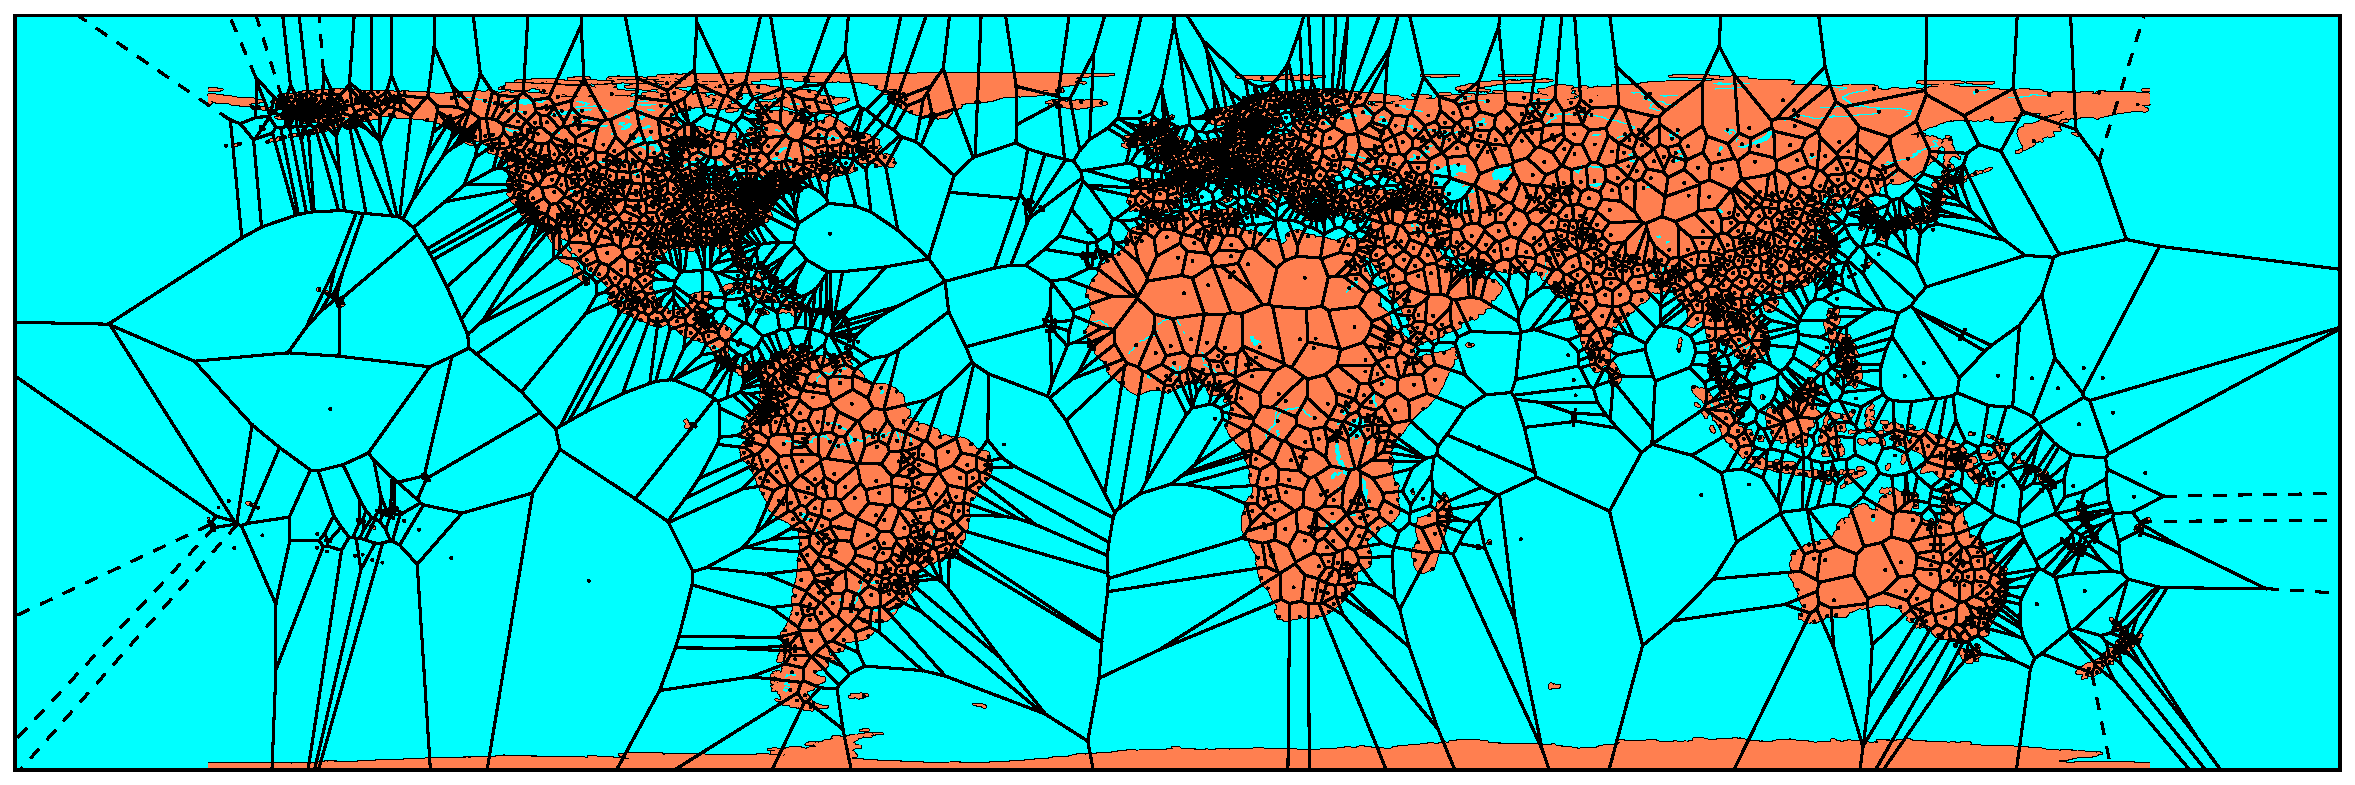
\includegraphics[width=1.0 \textwidth]{plots/voronoi.pdf}
	\caption{Voronoi tesselation based on airport locations. Airports are marked with a dot, region boundaries with lines and dashed lines.}
\end{figure}

